%% Run LaTeX on this file several times to get Table of Contents,
%% cross-references, and citations.

\documentclass[10pt]{book}
\usepackage{gvv-book}
%\usepackage{Wiley-AuthoringTemplate}
%\usepackage[sectionbib,authoryear]{natbib}% for name-date citation comment the below line
\usepackage[sectionbib,numbers]{natbib}% for numbered citation comment the above line

%%********************************************************************%%
%%       How many levels of section head would you like numbered?     %%
%% 0= no section numbers, 1= section, 2= subsection, 3= subsubsection %%
\setcounter{secnumdepth}{3}
%%********************************************************************%%
%%**********************************************************************%%
%%     How many levels of section head would you like to appear in the  %%
%%				Table of Contents?			%%
%% 0= chapter, 1= section, 2= subsection, 3= subsubsection titles.	%%
\setcounter{tocdepth}{2}
%%**********************************************************************%%

%\includeonly{ch01}
\makeindex

\begin{document}

\frontmatter
%%%%%%%%%%%%%%%%%%%%%%%%%%%%%%%%%%%%%%%%%%%%%%%%%%%%%%%%%%%%%%%%
%% Title Pages
%% Wiley will provide title and copyright page, but you can make
%% your own titlepages if you'd like anyway
%% Setting up title pages, type in the appropriate names here:

\booktitle{The Navic Standard}

\subtitle{Through Python}

\AuAff{G. V. V. Sharma}


%% \\ will start a new line.
%% You may add \affil{} for affiliation, ie,
%\authors{Robert M. Groves\\
%\affil{Universitat de les Illes Balears}
%Floyd J. Fowler, Jr.\\
%\affil{University of New Mexico}
%}

%% Print Half Title and Title Page:
%\halftitlepage
\titlepage

%%%%%%%%%%%%%%%%%%%%%%%%%%%%%%%%%%%%%%%%%%%%%%%%%%%%%%%%%%%%%%%%
%% Copyright Page

\begin{copyrightpage}{2023}
%Title, etc
\end{copyrightpage}

% Note, you must use \ to start indented lines, ie,
% 
% \begin{copyrightpage}{2004}
% Survey Methodology / Robert M. Groves . . . [et al.].
% \       p. cm.---(Wiley series in survey methodology)
% \    ``Wiley-Interscience."
% \    Includes bibliographical references and index.
% \    ISBN 0-471-48348-6 (pbk.)
% \    1. Surveys---Methodology.  2. Social 
% \  sciences---Research---Statistical methods.  I. Groves, Robert M.  II. %
% Series.\\

% HA31.2.S873 2004
% 001.4'33---dc22                                             2004044064
% \end{copyrightpage}

%%%%%%%%%%%%%%%%%%%%%%%%%%%%%%%%%%%%%%%%%%%%%%%%%%%%%%%%%%%%%%%%
%% Only Dedication (optional) 

%\dedication{To my parents}

\tableofcontents

%\listoffigures %optional
%\listoftables  %optional

%% or Contributor Page for edited books
%% before \tableofcontents

%%%%%%%%%%%%%%%%%%%%%%%%%%%%%%%%%%%%%%%%%%%%%%%%%%%%%%%%%%%%%%%%
%  Contributors Page for Edited Book
%%%%%%%%%%%%%%%%%%%%%%%%%%%%%%%%%%%%%%%%%%%%%%%%%%%%%%%%%%%%%%%%

% If your book has chapters written by different authors,
% you'll need a Contributors page.

% Use \begin{contributors}...\end{contributors} and
% then enter each author with the \name{} command, followed
% by the affiliation information.

% \begin{contributors}
% \name{Masayki Abe,} Fujitsu Laboratories Ltd., Fujitsu Limited, Atsugi, Japan
%
% \name{L. A. Akers,} Center for Solid State Electronics Research, Arizona State University, Tempe, Arizona
%
% \name{G. H. Bernstein,} Department of Electrical and Computer Engineering, University of Notre Dame, Notre Dame, South Bend, Indiana; formerly of
% Center for Solid State Electronics Research, Arizona
% State University, Tempe, Arizona 
% \end{contributors}

%%%%%%%%%%%%%%%%%%%%%%%%%%%%%%%%%%%%%%%%%%%%%%%%%%%%%%%%%%%%%%%%
% Optional Foreword:

%\begin{foreword}
%\lipsum[1-2]
%\end{foreword}

%%%%%%%%%%%%%%%%%%%%%%%%%%%%%%%%%%%%%%%%%%%%%%%%%%%%%%%%%%%%%%%%
% Optional Preface:

%\begin{preface}
%\lipsum[1-1]
%\prefaceauthor{}
%\where{place\\
% date}
%\end{preface}

% ie,
% \begin{preface}
% This is an example preface.
% \prefaceauthor{R. K. Watts}
% \where{Durham, North Carolina\\
% September, 2004}

%%%%%%%%%%%%%%%%%%%%%%%%%%%%%%%%%%%%%%%%%%%%%%%%%%%%%%%%%%%%%%%%
% Optional Acknowledgments:

%\acknowledgments
%\lipsum[1-2]
%\authorinitials{I. R. S.}  

%%%%%%%%%%%%%%%%%%%%%%%%%%%%%%%%
%% Glossary Type of Environment:

% \begin{glossary}
% \term{<term>}{<description>}
% \end{glossary}

%%%%%%%%%%%%%%%%%%%%%%%%%%%%%%%%
%\begin{acronyms}
%\acro{ASTA}{Arrivals See Time Averages}
%\acro{BHCA}{Busy Hour Call Attempts}
%\acro{BR}{Bandwidth Reservation}
%\acro{b.u.}{bandwidth unit(s)}
%\acro{CAC}{Call / Connection Admission Control}
%\acro{CBP}{Call Blocking Probability(-ies)}
%\acro{CCS}{Centum Call Seconds}
%\acro{CDTM}{Connection Dependent Threshold Model}
%\acro{CS}{Complete Sharing}
%\acro{DiffServ}{Differentiated Services}
%\acro{EMLM}{Erlang Multirate Loss Model}
%\acro{erl}{The Erlang unit of traffic-load}
%\acro{FIFO}{First in - First out}
%\acro{GB}{Global balance}
%\acro{GoS}{Grade of Service}
%\acro{ICT}{Information and Communication Technology}
%\acro{IntServ}{Integrated Services}
%\acro{IP}{Internet Protocol}
%\acro{ITU-T}{International Telecommunication Unit -- Standardization sector}
%\acro{LB}{Local balance}
%\acro{LHS}{Left hand side}
%\acro{LIFO}{Last in - First out}
%\acro{MMPP}{Markov Modulated Poisson Process}
%\acro{MPLS}{Multiple Protocol Labeling Switching}
%\acro{MRM}{Multi-Retry Model}
%\acro{MTM}{Multi-Threshold Model}
%\acro{PASTA}{Poisson Arrivals See Time Averages}
%\acro{PDF}{Probability Distribution Function}
%\acro{pdf}{probability density function}
%\acro{PFS}{Product Form Solution}
%\acro{QoS}{Quality of Service}
%\acro{r.v.}{random variable(s)}
%\acro{RED}{random early detection}
%\acro{RHS}{Right hand side}
%\acro{RLA}{Reduced Load Approximation}
%\acro{SIRO}{service in random order}
%\acro{SRM}{Single-Retry Model}
%\acro{STM}{Single-Threshold Model}
%\acro{TCP}{Transport Control Protocol}
%\acro{TH}{Threshold(s)}
%\acro{UDP}{User Datagram Protocol}
%\end{acronyms}

\setcounter{page}{1}

\begin{introduction}
This book introduces the NAVIC communication standard through Python exercises

\end{introduction}

\mainmatter
\chapter{Design Parameters}
\section{The Frequency Bands}

\chapter{Channel Modelling}
The phenomena modelled in the satellite communication channel are Doppler shift, delay, power scaling and receiver noise.
\section{Doppler shift}
Due to relative motion between the satellites and the receiver, the transmitted signals undergo a frequency shift before arriving at the receiver. This shift%
in frequency is called Doppler shift and can be computed as
\begin{equation}
    f_{shift} = f_{d}-f_{c} = \brak{\frac{V_{rel}}{c-V_{S,dir}}}f_{c}  
\end{equation}
where,

$f_{Shift}$ = Frequency shift due to Doppler

$f_{d}$ = Frequency observed at receiver

$f_{c}$ = Carrier frequency at transmitter

$V_{rel}$ = Relative velocity of transmitter and receiver

$V_{S,dir}$ = Velocity of satellite along radial direction

$c$ = Speed of light

$V_{rel}$ is given by
\begin{align}
    V_{rel} &= V_{S,dir} - V_{R,dir}
\end{align}
where,

$V_{R,dir}$ = Velocity of receiver along radial direction

$V_{R,dir}$ and $V_{S,dir}$ are given by
\begin{align}
    V_{R,dir} &= \vec{V}_{R} \cdot \hat{\vec{dir}}\\
    V_{D,dir} &= \vec{V}_{S} \cdot \hat{\vec{dir}}
\end{align}
where,

$\hat{\vec{dir}}$ = Unit vector from satellite to receiver i.e. radial direction

$\vec{V_{S}}$ = Velocity of satellite

$\vec{V_{R}}$ = Velocity of receiver

$\hat{\vec{dir}}$ is given by
\begin{align}
    \hat{\vec{dir}} = \frac{\vec{P_{S}}-\vec{P_{R}}}{\norm{\vec{P_{S}}-\vec{P_{R}}}}
\end{align}
where,

$\vec{P_{S}}$ = Position of satellite

$\vec{P_{R}}$ = Position of receiver


The Doppler shift is introduced by muliplying the satellite signal with a complex exponential,
\begin{equation}
    x_{Shift}\sbrak{n} = x\sbrak{n}e^{-2 \pi j \brak{f_{c}+f_{Shift}} n t_{s}}
\end{equation}
where,

$x_{Shift}\sbrak{n}$ = Doppler shifted signal

$x\sbrak{n}$ = Satellite signal

$t_{s}$ = Sampling period

\section{Delay}
Since there is a finite distance between the satellite and the receiver, the signal at the reciever is a delayed version of the transmitted signal. This delay is given by
\begin{equation}
    D_{s} = \frac{d}{c}f_{s} 
\end{equation}
where,

$D_{s}$ = Total delay in samples

$d$ = Distance between satellite and receiver

$c$ = Speed of light

$f_{s}$ = Sampling rate

The total delay on the satellite signal is modeled in two steps. First, a static delay is modeled which does not change with time and it is always an integer number of samples. Then, %
a variable delay is modeled which can be a rational number of samples. While modelling the static delay, the entire delay is not introduced so that variable delay modelling handles the remaining %
delay.

To introduce the static delay, the samples are read from a queue whose size is the desired static delay length. When samples are read from the queue, an equal number of new samples are %
updated in the queue. To introduce the variable delay, the signal is passed through an all-pass FIR filter with an almost constant phase response. Its coefficients are calculated %
using the delay value required.

\section{Power Scaling}
When a transmitting antenna transmits radio waves to a receiving antenna, the radio wave power received is given by,
\begin{equation}
    P_r = P_t D_t D_r \brak{\frac{1}{4 \pi \brak{f_c + f_{Shift}} D}}^2
\end{equation}
where,

$P_r$ = Received power

$P_t$ = Transmitted power

$D_t$ = Directivity of transmitting antenna 

$D_r$ = Directivity of receiving antenna 

$D$ = Total delay in seconds

To scale the received signal as per the received power calculated,
\begin{equation}
    x_{Scaled}\sbrak{n} = \frac{\sqrt{P_r}}{\operatorname{rms}\brak{x\sbrak{n}}}x\sbrak{n}
\end{equation}   

\section{Receiver noise}

\chapter{Transmitter}

\section{Frame structure}
NavIC master frame consists of 2400 symbols, divided to four subframes. Each subframe is 600 symbols long. Subframes 1 and 2 transmit fixed navigation parameters. Subframe 3 and 4 transmit secondary navigation parameters in the form of messages. Each subframe is 292 bits long without FEC encoding and sync word. It starts with TLM word of 8 bits. Ends with 24 bit Cyclic Redundancy Check(CRC) followed by 6 tail bits. In subframes 1 and 2 navigation data is alloted 232 bits, starting from bit 31. In subframe 3 and 4, 220 bits are alloted starting from bit 37. For detailed structure of subframes, refer to chapter 5.9 in the doc
\subsection{Cyclic Redundancy Check(CRC)}
The parity coding of data signal follows 24Q polynomial for each subframe. 24 bits of CRC parity will provide protection against burst as well as random errors with undetected eroor probability of $2^{-24}$ for all channel bit error probabilities 0.5
\begin{equation}
    g(X) = \sum_{i = 0}^{24}g_{i}X^i\;\;
    g_{i}=1\; for\; i = 0,1,3,4,5,6,7,10,11,14,17,18,23,24
\end{equation}
\section{Encoding}
The navigation data subframe of 292 bits is rate 1/2 convolution encoded and clocked at 50 symbols per second. Each subframe of 292 bits after encoding results in 584 bits. For parameters and coding scheme, refer to below doc
\subsection{Interleaving}
Any burst errors during the data transmission can be corrected by interleaving. In matrix interleaving, input symbols are filled into a matrix column wise and read at the output row wise. This will spread the burst error, if any, during the transmission. For SPS, data is filled into matrix of size 73 by 8(73 columns, 8 rows).
\subsection{Sync word and Tail bits}
Each subframe has a 16 bit word synchronization pattern which is not encoded. Sync pattern is EB90 Hex. Tail bit consists of 6 zero value bits enabling completion of FEC decoding of each subframe in the receiver.

\section{Modulation}
\subsection{Standard Positioning Service}
The SPS signal is BPSK(1) modulated on L5 and S bands. The navigation data at data rate of 50 sps (1/2 rate FEC encoded) is modulo 2 added to PRN code chipped at 1.023 Mcps. The CDMA modulated code, modulates the L5 and S carriers at 1176.45 MHz and 2492.028 MHz respectively.
\subsection{Pseudo Random Noise codes(PRN)}
NavIC uses Gold codes fo SPS signal. They are generated using Linear Feedback Shift Registers. For L5 and S band, the code length is 1ms and consists of 1023 chips. The code is chipped at 1.023 Mcps. Two polynomials G1 and G2 are used to generate the gold code sequence. G2's initial state provides unique PRN code for each satellite. All bits of G1 are initialized as 1. G1 and G2 are XOR'ed to generate final 1023 chip long PRN sequence, the time period being 1ms. For more information refer to chapter 4 in the doc.
\subsection{Baseband Modulation}
The carrier signal is modulated by BPSK(1), Data channel BOC(5,2), and Pilot Channel BOC(5,2). To have a constant envelop when passed through power amplifier, we add additional signal called interplex signal.
For detailed mathematical equations, refer to chapter 3.3 in the below document

\chapter{Computing the Position and Velocity of the satellite from the RINEX file}
\section{Introduction}
In order to achieve the navigation services we have to find the position and velocity of satellite in its orbit.In order to find the position and velocity we have the source called RINEX file Which contains all the orbital parameters of the satellite in its orbit.In this document we  compute the position and velocity of GPS and NAVIC satellites.The RINEX files is different for both the satellites but the algorithm for finding the position and velocity is same.
\section{Determination of satellite position}
RINEX files will be available in official websites for all the satellites.The RINEX files contains all the information of the orbital parameters of the particular satellite.The Orbital elements of satellite from rinex file is given in below table.
\subsection{Orbital parameters in rinex file}
\begin{tabular}{ | m{10em} | m{10cm} | } 
  \hline
  $\sqrt{a}$   & Square rooot of semimajor axis \\
  \hline
  e & 
  Eccentricity \\  
  \hline
  $\Delta$n & Mean motion diffeerence from computed value  \\
  \hline
  $M_0$ & Mean anom
  maly at reference time \\
  \hline
  $\Omega_0$ & Longitude of ascending node
  n
  of orbit plane at weekly epoch  \\
  \hline
  $i_0$ & Inclination angle
  a
  at reference time   \\
  \hline
  w & Argum
  ment of perigee \\
  \hline
$\Omega_.$& Rate of right ascension  \\
  \hline
  IDOT & Rate off inclination angle  \\
  \hline
$t_{oe}$  & Ephemeeris reference time  \\
  \hline
  IODE  &  Issue of data, ephemeris \\
  \hline
  $C_{uc}$ & Amplitude of cosine harmonic
  h
  correction term to the
  argum
  ment of latitude   \\
  \hline
  $C_{us}$& Amplitude of sine harmonnic correction term to the argument
  of latitude \\
  \hline
  $C_{rc}$  &  Amplitude of cosine harrmonic correction term to the orbit
  radius \\
  \hline
  $C_{rs}$ & Amplitude of sine harm
  monic correction term to the orbit
  radius  \\
  \hline
  $C_{ic}$ & Amplitude of cosine harm
  monic correction term to the angle of
  i
  inclination \\
  \hline
  $C_{is}$ & Amplitude of sine harmoonic correction term to the angle of
  i
  inclination  \\
  \hline
\end{tabular}
\begin{figure}
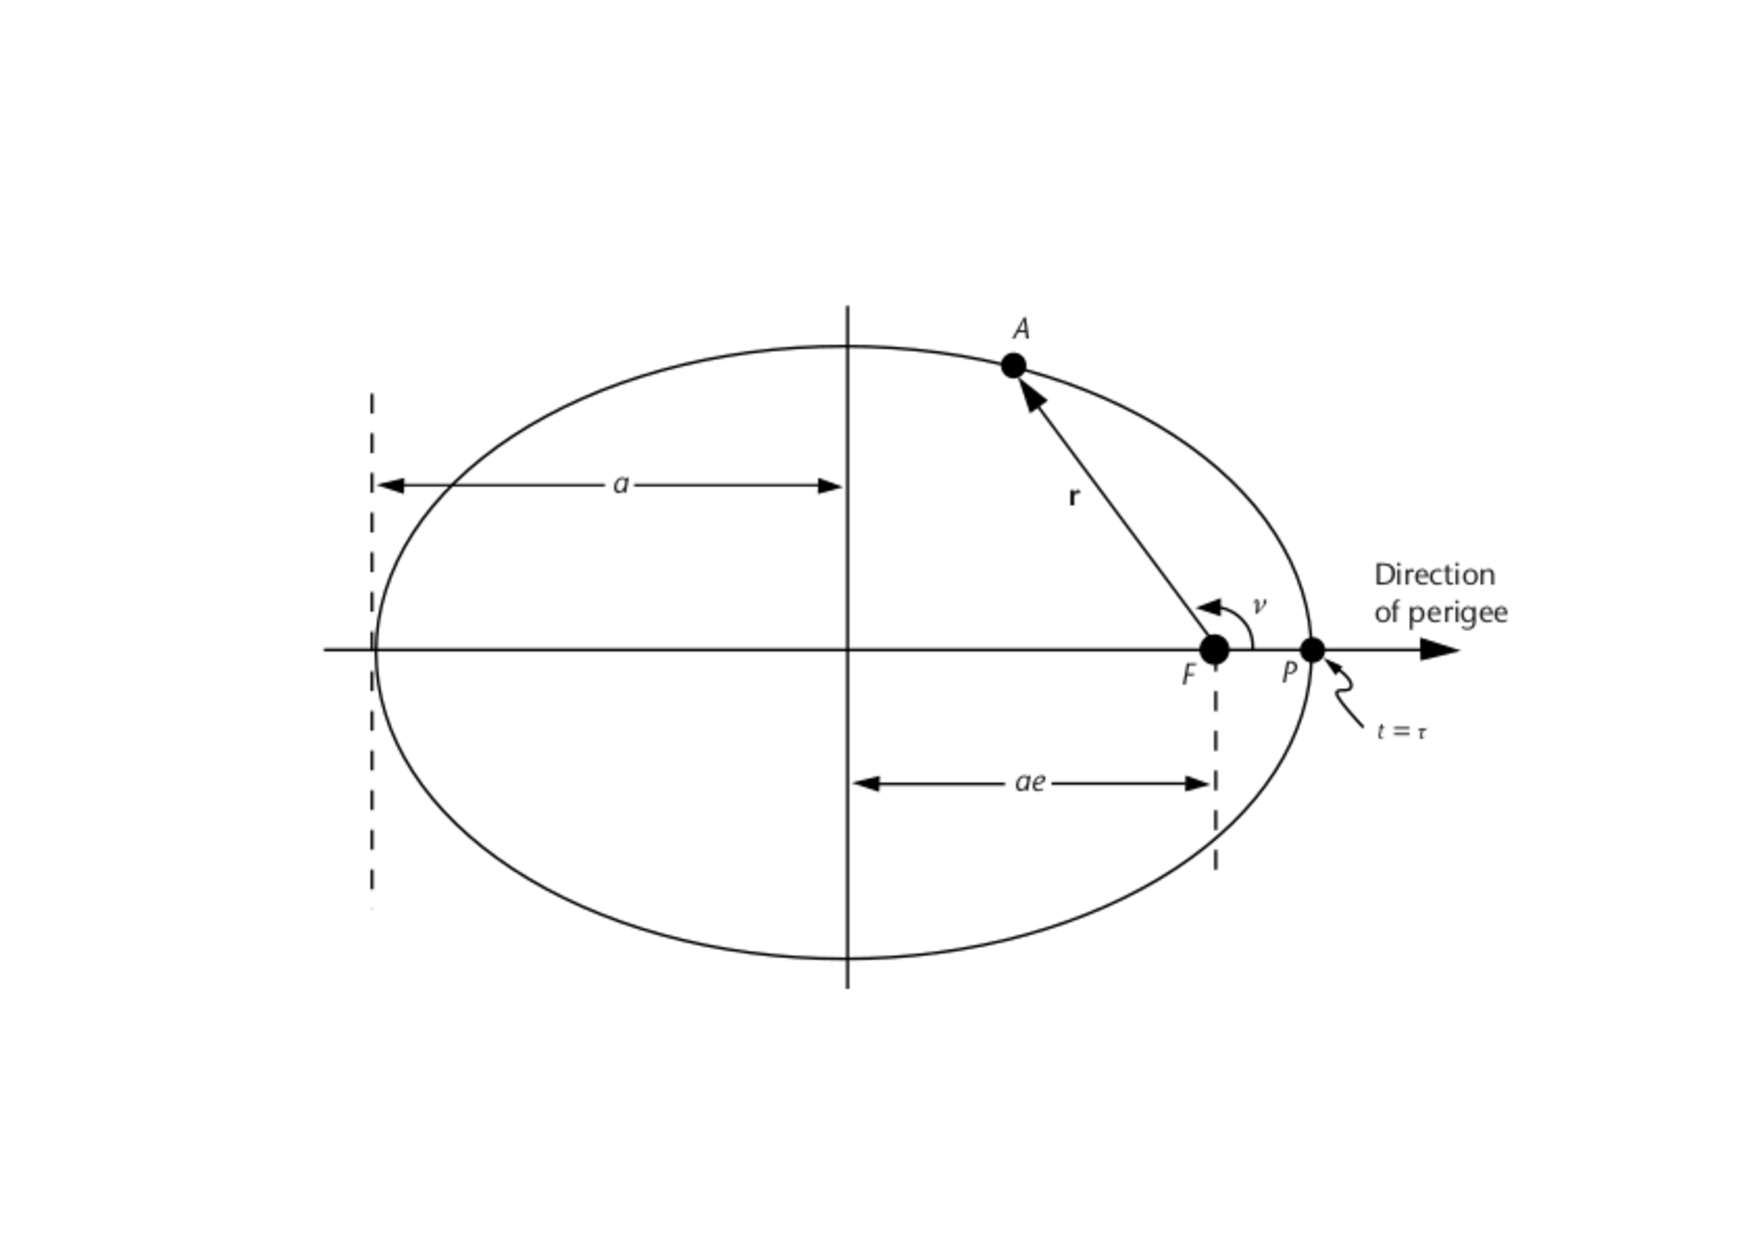
\includegraphics[scale=0.4]{./figs/1.pdf}
\end{figure}
\vspace{30cm}
\\
In the above Figure 
\begin{enumerate}
\item The elliptical orbit has a focus at point
F, which corresponds to the center of the mass of the Earth.
\item The time t0 at which the satellite is at some
reference point A in its orbit is known as the epoch.
\item The point, P, where the satellite is closest to the center of the Earth
is known as perigee.
\item The time at which the satellite passes perigee,t, is another
Keplerian orbital parameter.
\end{enumerate}
\vspace{5mm}
The three Keplerian orbital elements
that define the shape of the elliptical orbit and time relative to perigee are as
follows:
\begin{enumerate}
  \item a = Semimajor axis of the ellipse
  \item e = eccentricity of the ellipse
  \item t = time of perigee passage
\end{enumerate}
In order to find the position of satellite let us understand the keplerian orbital elements.\\
\\
\textbf{True anamoly :} The angle in the orbital plane measured counterclockwise from
the direction of perigee to the satellite.\\ 
\\
\textbf{Eccentric anamoly :} Geometrically, the eccentric anomaly is constructed from the true anom-
aly first by circumscribing a circle around the elliptical orbit. Next, a perpendicular
is dropped from the point A on the orbit to the major axis of the orbit, and this per-
pendicular is extended upward until it intersects the circumscribed circle at point B. The angle measured at the center of the circle, O, counter-
clockwise from the direction of perigee to the line segment.
\begin{figure}
  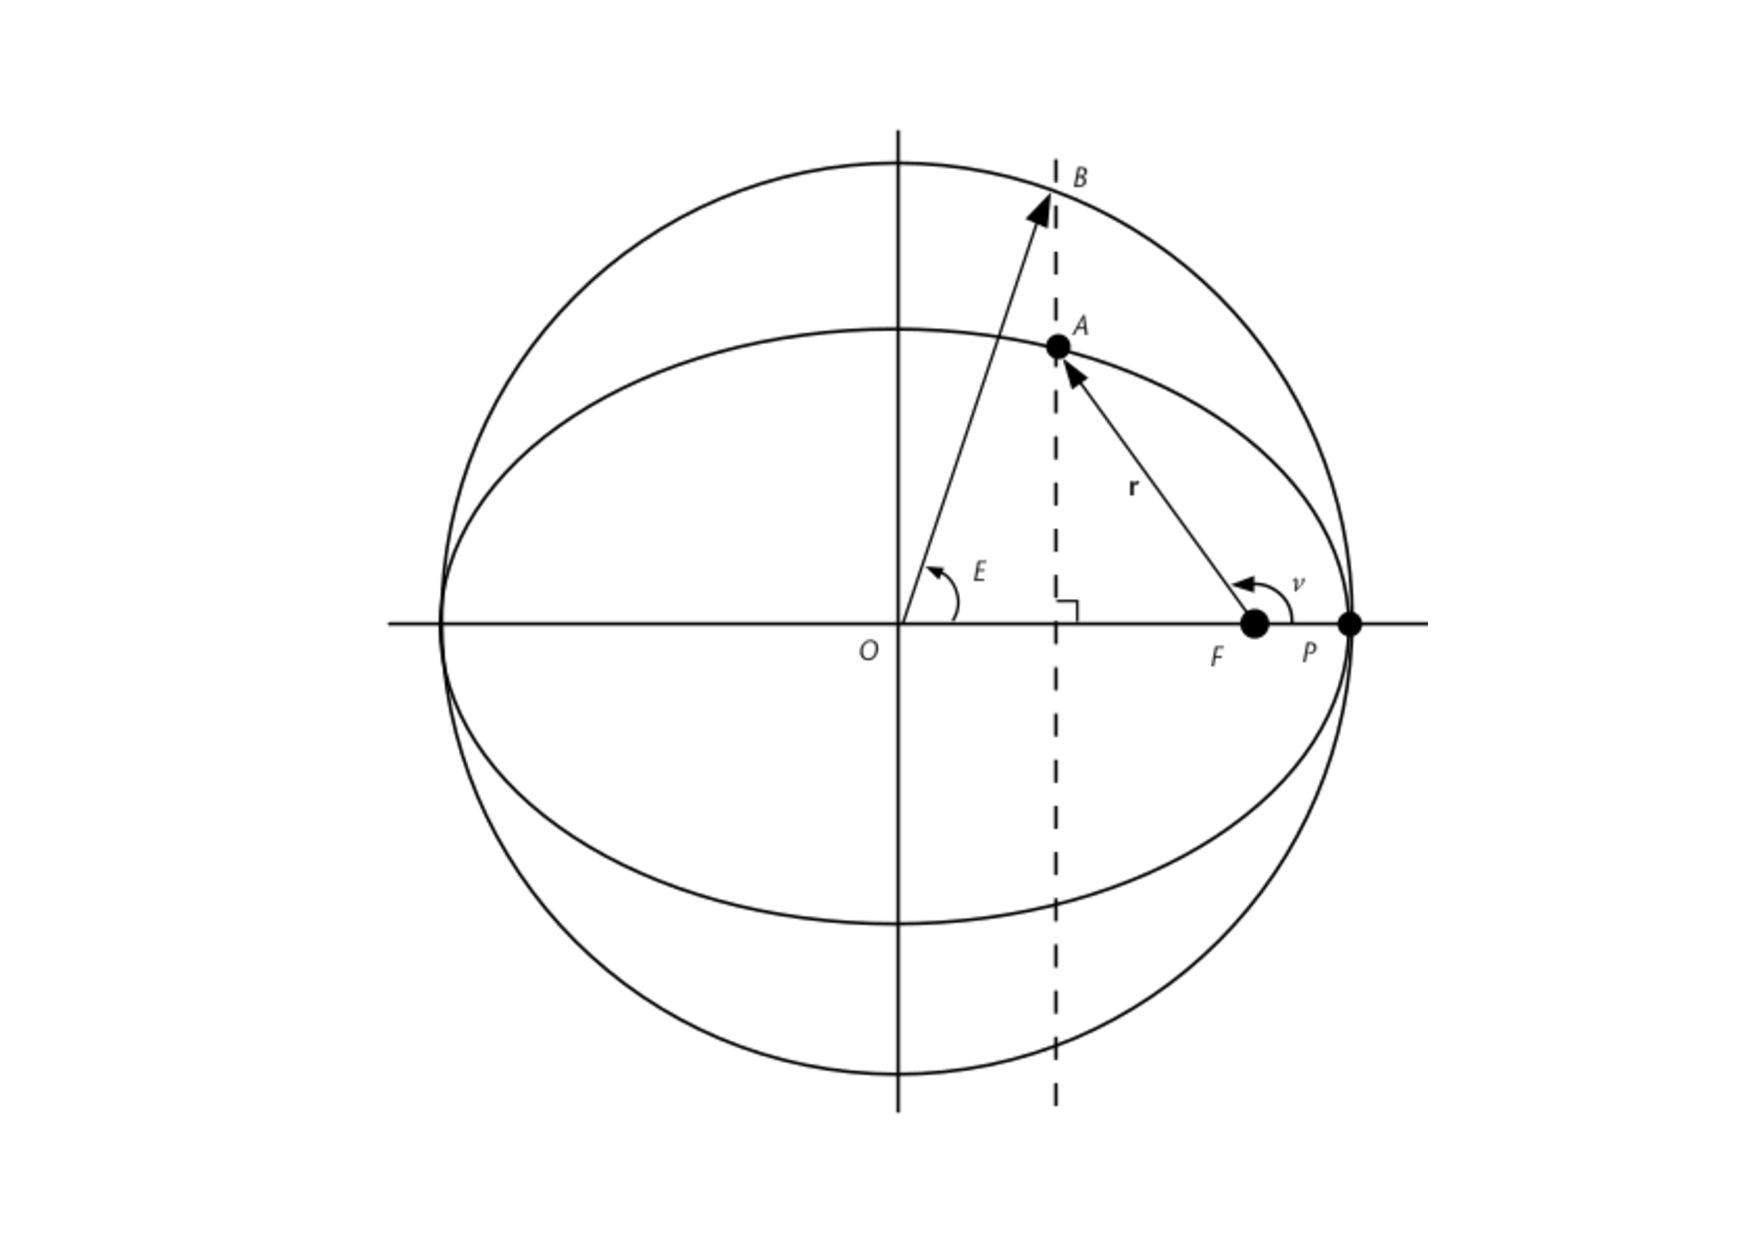
\includegraphics[scale=0.4]{./figs/2.pdf}
  \end{figure}
 \begin{align}
E&=2\arctan (\sqrt{\frac{1+e}{1-e}}\tan(\frac{v}{2})  )
 \end{align}
 \\
 \textbf{Mean anamoly :} The importance of transforming from the true to the mean
 anomaly is that time varies linearly with the mean anomaly.\\
 \begin{align}
  M&=M_o+n*(t-t_o)
 \end{align}
 Where,\\
 $M_o$ is Mean anamoly at the time of epch.\\
 M is the mean anomaly at time t.\\
 \begin{align}
  n&=\sqrt{\frac{\mu }{a^3}} \\
  \mu&=398,600.5 * 10^8 m^3/s^2
 \end{align} 
 \\
 In the case of GPS or Navic, the Keplerian
parameters are defined in relation to the ECEF coordinate system .In this case, the xy-plane is always the Earth's equatorial plane.
The following three Keplerian orbital elements define the orientation of the orbit in the
ECEF coordinate system:\\
\\
\textbf{Inclination of orbit :} Inclination is the dihedral angle between the Earth’s equatorial plane and the
satellite’s orbital plane.\\
\\
\textbf{longitude of the ascending node :} The orbital element that defines the
angle between the +x-axis and the direction of the ascending node is called the right
ascension of the ascending node (RAAN). Because the +x-axis is fixed in the direc-
tion of the prime meridian (0° longitude) in the ECEF coordinate system, the right
ascension of the ascending node is actually the longitude of the ascending node,$\Omega$.\\
\\
\textbf{Arguement of perigee :} Measures the angle
from the ascending node to the direction of perigee in the orbit. \\
\\
Notice that $\Omega$ is measured in the equatorial plane, whereas $\omega$ is measured in the orbital plane.
The following formulas are used for computing the position,velocity of the satellite in the elliptical orbit.Where the inputs are taken from the rinex file.
\begin{align}
  \Omega^. &= 7.2921151467*10^{-5} rad/sec \\
  a&=\sqrt{a^2} \\
  t_k&=t-t_oe \\
  n&=n_o+\Delta n \\
  M_k&=M_o+nt_k \\
  E_k&=M_k+e\sin(E_k) \\
  \sin(v_k) &=\frac{1 - e^2sin E_k}{1 - ecos E_k}\\
\cos(v_k)&=\frac{\cos(E_K)-e}{1-ecos(E_k)} \\
\phi_k&=v_k+w \\
\delta \phi_k &= C_{us}\sin(2 \phi_k ) + C_{uc}\cos(2 \phi_kk ) \\
\delta r_k &= C_{rs}\sin(2 \phi_k ) + C_{rc}\cos(2 \phi_k ) \\
\delta i_k &= C_{is}\sin(2 \phi_k ) + C_{ic}\cos(2 \phi_k ) \\
u_k&= \phi_k + \delta \phi_k \\
r_k &= a(1 - e\cos E_k ) + \delta r_k \\
i_k &= i_0 + \frac{di}{dt}t_k + \delta i_k \\
\Omega_k &= \Omega_0 + \Omega^. - \Omega_e^. (t_k ) - \Omega_e^. t_{oe} \\
x_p &= r_k \cos(u_k) \\
y_p &= r_k \sin(u_k) \\
x_s &= x_p \cos \Omega_k - y_p \cos i_k \sin \Omega_k \\
y_s &= x_p \sin \Omega_k - y_p \cos i_k \cos \Omega_k \\
z_s &= y_p \sin i_k
\end{align}
\\
By computing the above formulas [$x_s,y_s,z_s$] are the position of satellite in ECEF cooedinate frame.\\
The velocity of the satellite is obtained by differentiating the above position equations with respect to time.The final equation is as follows: 
\\
\\
$x_v = -x_p \Omega_k^. \sin \Omega_k + x_p^. \cos \Omega_k - y_p^. \sin \Omega_k \cos i_k$ \\
$-y_p(\Omega_k^.\cos \Omega_k \cos i_k - \frac{dik}{dt} \sin \Omega_k \sin i_k )$ \\
\\
$y_v = -x_p \Omega_k^. \cos \Omega_k + x_p^. \sin \Omega_k - y_p^. \cos \Omega_k \cos i_k$ \\
$-y_p(\Omega_k^.\sin \Omega_k \cos i_k - \frac{dik}{dt} \cos \Omega_k \sin i_k )$ \\
\\
$z_v = y_p\frac{di_k}{dt}\cos i_k + y_p^.\sin i_k$
\\
\\
By computing the above formulas $[x_v,y_v,z_v]$ is the velocity vector of satellite in ECEF coordinate frame. 
\\
\\
\textbf{Computations of error corrections :} 
\begin{enumerate}
  \item \textbf{Clock Correction :} \\
One of the largest sources of error in calculating range is
satellite clock error. To get the accuracy of the receiver
position signal transmission and reception time must be
precisely known. Because of the travel time of light, one
nanosecond of inaccuracy in the clock causes 30 centimeter
error in position. Satellite clock correction coefficients - clock
bias, clock drift, and clock drift rate are obtained from the
RINEX Navigation file. Calculation of the satellite clock error
is given by 
\begin{align}
\Delta t_{clk}&=a_{f0} + a_{f1}(t-t_{oc}) + a_{f2}(t-t_{oc})^2
\end{align}
where ,\\
$\Delta t_{clk}$ is clock offset in seconds.\\
t is IRNSS system time at transmission in seconds.\\
$t_{oc}$ is clock data reference time. \\
$a_{f0}$ is clock bias. \\
$a_{f1}$ is clock drift.\\
$a_{f2}$ is clock drift rate.
\item \textbf{Relativistic Correction :} \\
Because of the high speed of satellites and
weaker gravity, clocks on the satellites run a little faster than the clock on the Earth. Error found because the relativity is in
nanoseconds. The computation of relativistic clock error is given
by
\begin{align}
\delta _{rel}&=Fe\sqrt{a}\sin (E)
\end{align}
where ,\\
a is semimajor axis of the ellipse. \\
e is eccentricity of the ellipse. \\
F is -4.442807633 * $10^{-10}$ \\
E is Eccentric anamoly.
$\delta _{rel}$ is relativistic clock correction \\
\end{enumerate}
\section{Computing the position and velocity of the  GPS satellite using python}
\textbf{Installations :}
\begin{enumerate}
\item pip3 install pymap3d
\item pip3 install georinex
\item pip3 install itertools
\item pip3 install argparse
\end{enumerate}
\textbf{Algorithm for finding the position and velocity of satellite From Rinex file :}
\begin{enumerate}
  \item Get the rinex file for GPS  satellite from the official website.
  \item The Rinex file contains the observational file and navigation file.
  \item Convert the Rinex file to CSV file using the python \\
  The below python function will convert the GPS RINEX file to CSV file.
  \begin{lstlisting}
    ./rinex_to_csv/funcs.py
  \end{lstlisting}
  \item Remove the empty rows in csv file.The python function for removing empty rows is 
  \begin{lstlisting}
    ./rinex_to_csv/funcs.py
  \end{lstlisting}
  \item Convert the csv file to list in python so that each row is corresponds to the parameters of the satellite. Function for converting the csv file to list is given as :
  \begin{lstlisting}
    ./rinexread/funcs.py
  \end{lstlisting} 
  \item Process the above list with the formulas mentioned in chaprter 2 \\
  The python function for finding the position of satellite is given as :
  \begin{lstlisting}
    ./position/funcs.py
  \end{lstlisting}
  \item The velocity of the satellte is computed by the function 
  \begin{lstlisting}
    ./velocity/funcs.py
  \end{lstlisting}
  \item The distance between the satellite and receiver is obtained by the python package called \textbf{pymap3d},using this package convert ECEF to spherical coordinate frame.So that we obtain the distance between satellite and receiver.
  \item These position and velocity of the satellite is used for computing the doppler shift.
\end{enumerate}
\vspace{5mm}
The above alogorith will work for both GPS and Navic sarellite.If there is a problem in converting Navic RINEX file to csv file then follow the instructions below:
\begin{enumerate}
\item go to the mentioned folder in your laptop.
\begin{lstlisting}
  ./home/mannava/.local/lib/python3.10/site-packages/georinex/nav3.py
\end{lstlisting}
\item Go to the line 220 in nav3.py file and modify the below changes.
\begin{lstlisting}
  elif numval == 29:  # only one trailing spare fields
            cf = cf[:-2]
        elif numval == 28:  # only one trailing spare fields
            cf = cf[:-3]
        elif numval == 27:  # only one trailing spare fields
            cf = cf[:-4]
        elif numval == 26:  # only one trailing spare fields
            cf = cf[:-5]
\end{lstlisting}
\end{enumerate}

























\backmatter
\appendix
%\chapter{ Filter Design}
%\input{filtdesign/writeup/filter_design.tex}

\latexprintindex

\end{document}

 
